\documentclass[11pt,a4paper]{report}
\usepackage[textwidth=37em,vmargin=30mm]{geometry}
\usepackage{calc,xunicode,amsmath,amssymb,paralist,enumitem,tabu,booktabs,datetime2,xeCJK,xeCJKfntef,listings}
\usepackage{tocloft,fancyhdr,tcolorbox,xcolor,graphicx,eso-pic,xltxtra,xelatexemoji}

\newcommand{\envyear}[0]{2024}
\newcommand{\envdatestr}[0]{2024-11-10}
\newcommand{\envfinaldir}[0]{webdb/2024/20241110/final}

\usepackage[hidelinks]{hyperref}
\hypersetup{
    colorlinks=false,
    pdfpagemode=FullScreen,
    pdftitle={Web Digest - \envdatestr}
}

\setlength{\cftbeforechapskip}{10pt}
\renewcommand{\cftchapfont}{\rmfamily\bfseries\large\raggedright}
\setlength{\cftbeforesecskip}{2pt}
\renewcommand{\cftsecfont}{\sffamily\small\raggedright}

\setdefaultleftmargin{2em}{2em}{1em}{1em}{1em}{1em}

\usepackage{xeCJK,xeCJKfntef}
\xeCJKsetup{PunctStyle=plain,RubberPunctSkip=false,CJKglue=\strut\hskip 0pt plus 0.1em minus 0.05em,CJKecglue=\strut\hskip 0.22em plus 0.2em}
\XeTeXlinebreaklocale "zh"
\XeTeXlinebreakskip = 0pt


\setmainfont{Brygada 1918}
\setromanfont{Brygada 1918}
\setsansfont{IBM Plex Sans}
\setmonofont{JetBrains Mono NL}
\setCJKmainfont{Noto Serif CJK SC}
\setCJKromanfont{Noto Serif CJK SC}
\setCJKsansfont{Noto Sans CJK SC}
\setCJKmonofont{Noto Sans CJK SC}

\setlength{\parindent}{0pt}
\setlength{\parskip}{8pt}
\linespread{1.15}

\lstset{
	basicstyle=\ttfamily\footnotesize,
	numbersep=5pt,
	backgroundcolor=\color{black!5},
	showspaces=false,
	showstringspaces=false,
	showtabs=false,
	tabsize=2,
	captionpos=b,
	breaklines=true,
	breakatwhitespace=true,
	breakautoindent=true,
	linewidth=\textwidth
}






\newcommand{\coverpic}[2]{
    % argv: itemurl, authorname
    Cover photo by #2~~(\href{#1}{#1})
}
\newcommand{\makeheader}[0]{
    \begin{titlepage}
        % \newgeometry{hmargin=15mm,tmargin=21mm,bmargin=12mm}
        \begin{center}
            
            \rmfamily\scshape
            \fontspec{BaskervilleF}
            \fontspec{Old Standard}
            \fontsize{59pt}{70pt}\selectfont
            WEB\hfill DIGEST
            
            \vfill
            % \vskip 30pt
            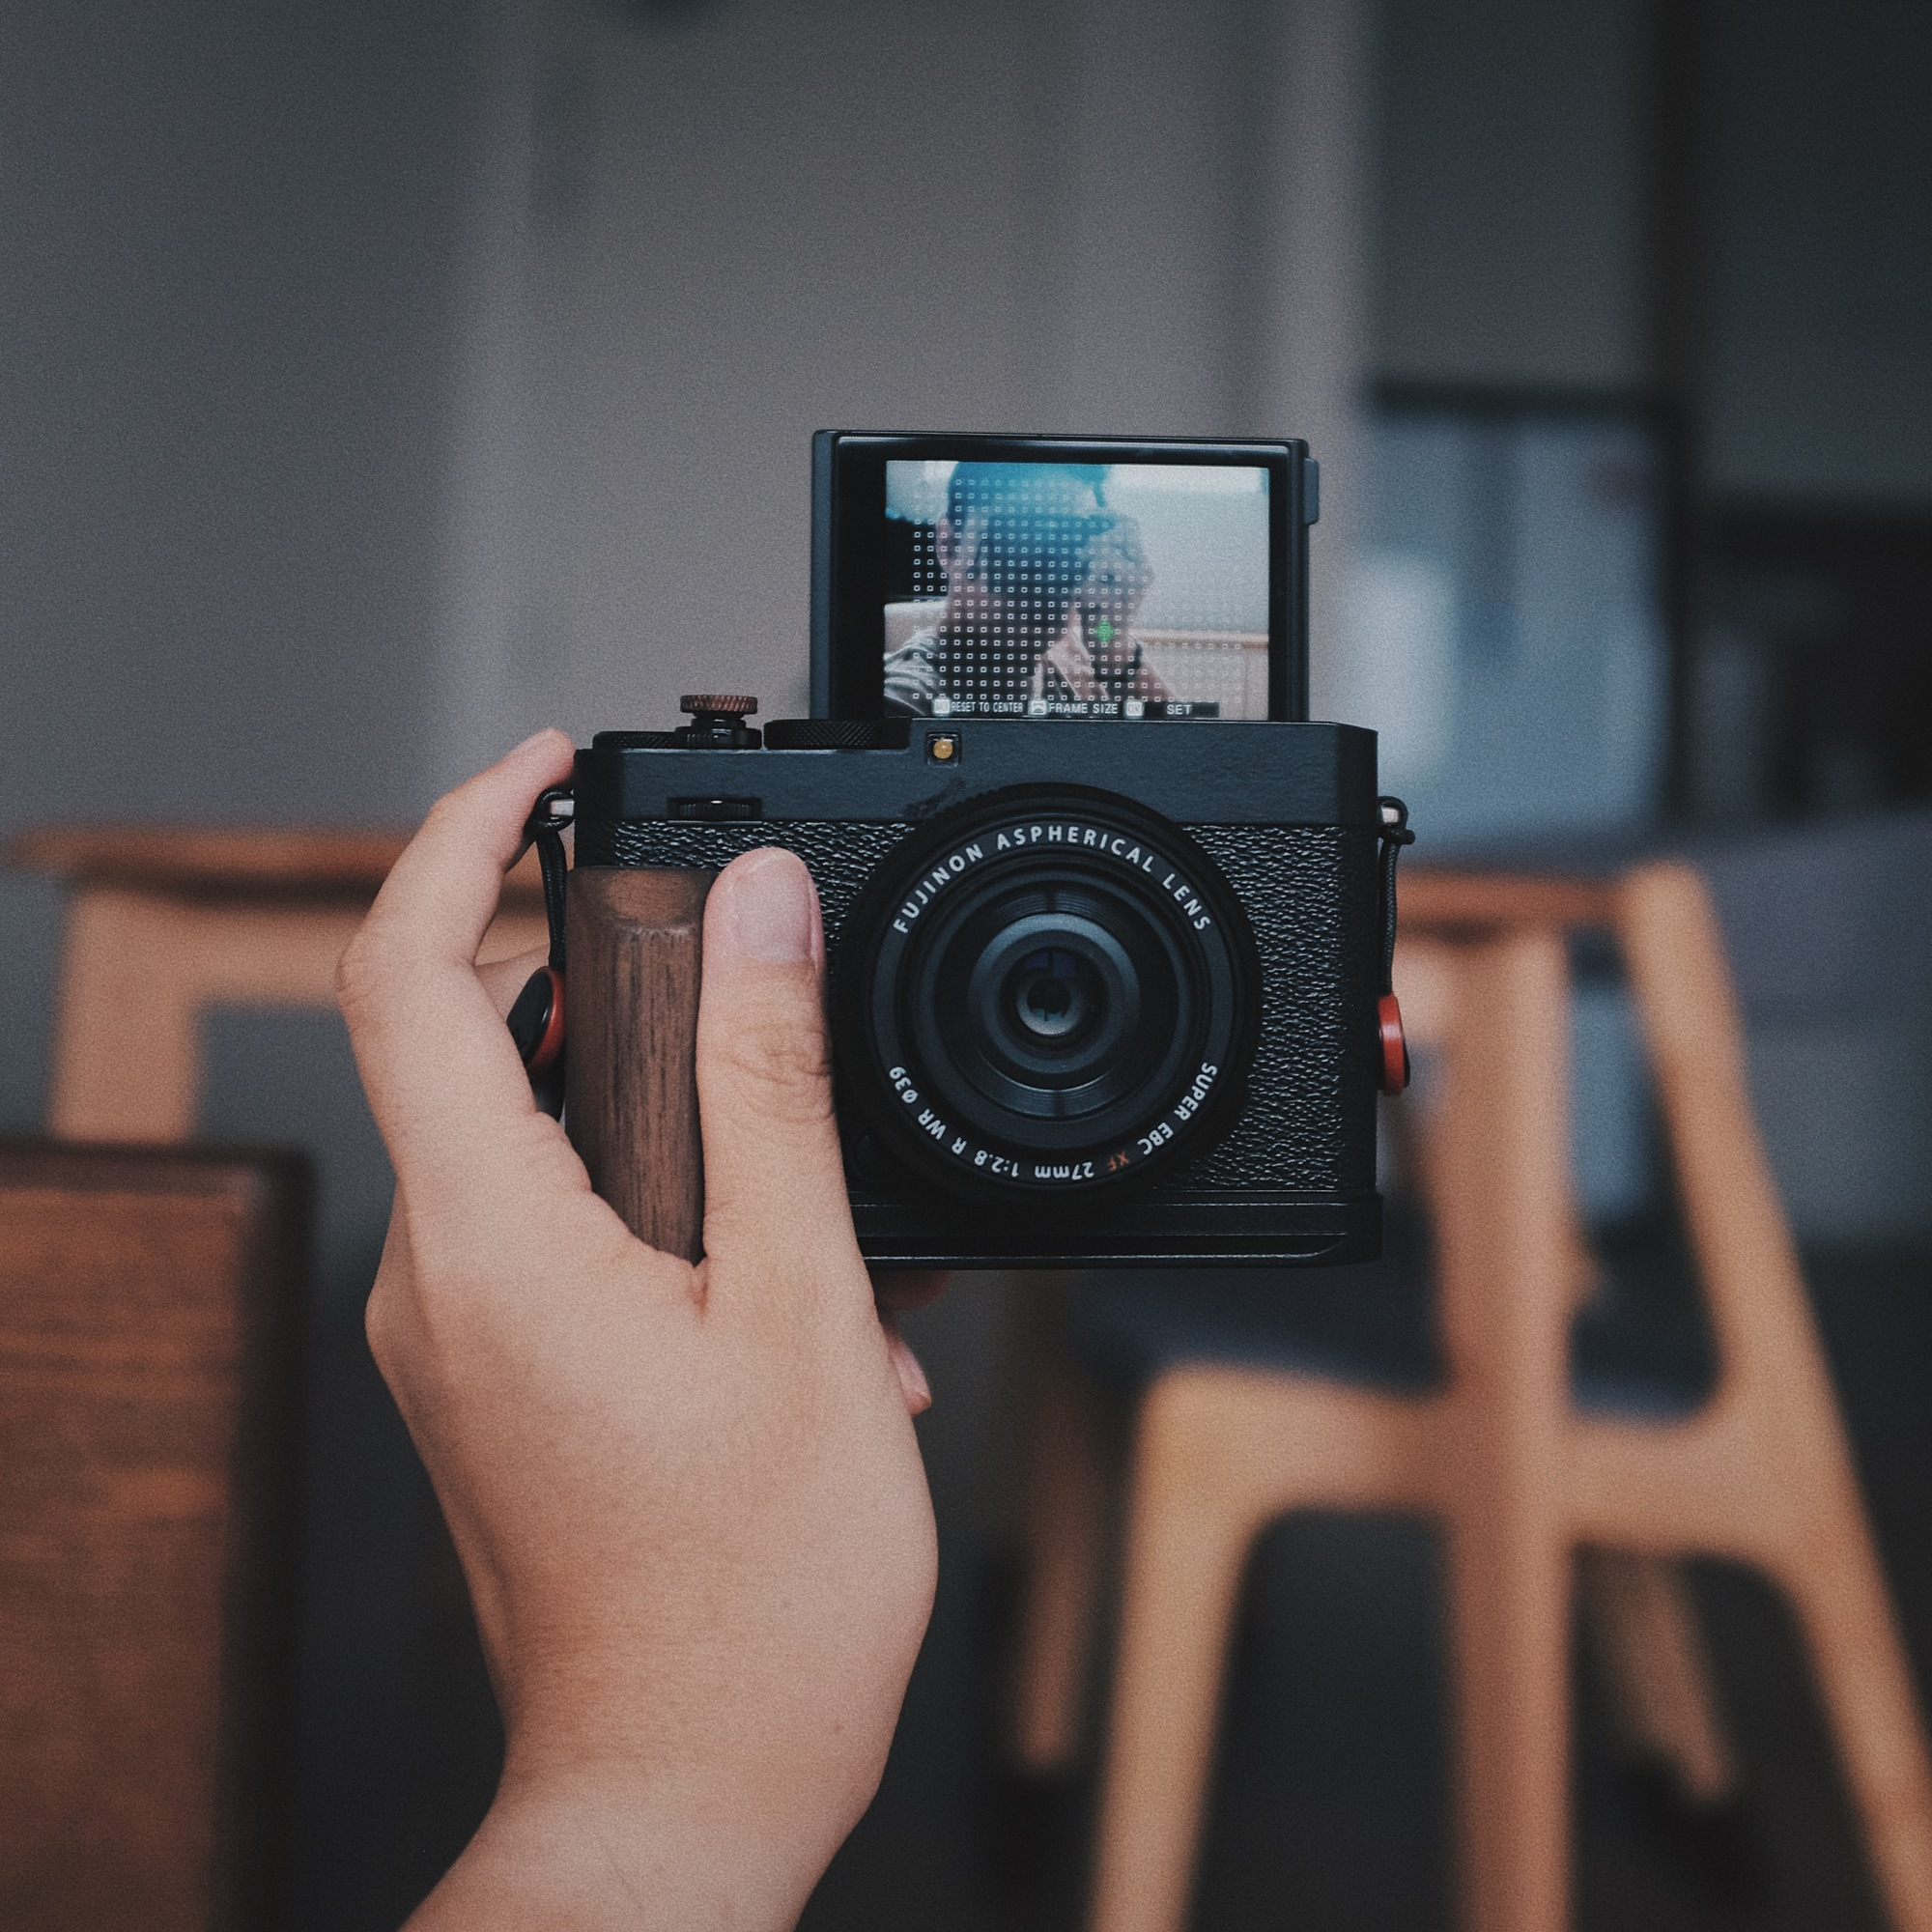
\includegraphics[width=\linewidth]{\envfinaldir/coverpic-prod.jpg}\par
            % \vskip 30pt
            \vfill

            \normalsize\rmfamily\scshape
            \copyright{} The Web Digest Project \hfill\large \envdatestr
        \end{center}
    \end{titlepage}
    % \restoregeometry
}
\newcommand{\simplehref}[1]{%
    \textcolor{blue!80!green}{\href{#1}{#1}}%
}
\renewcommand{\contentsname}{\center\Huge\sffamily\bfseries Contents\par\vskip 20pt}
\newcounter{ipartcounter}
\setcounter{ipartcounter}{0}
\newcommand{\ipart}[1]{
    % \vskip 20pt
    \clearpage
    \stepcounter{ipartcounter}
    \phantomsection
    \addcontentsline{toc}{chapter}{#1}
    % \begin{center}
    %     \Huge
    %     \sffamily\bfseries
    %     #1
    % \end{center}
    % \vskip 20pt plus 7pt
}
\newcounter{ichaptercounter}
\setcounter{ichaptercounter}{0}
\newcommand{\ichapter}[1]{
    % \vskip 20pt
    \clearpage
    \stepcounter{ichaptercounter}
    \phantomsection
    \addcontentsline{toc}{section}{\numberline{\arabic{ichaptercounter}}#1}
    \begin{center}
        \Huge
        \sffamily\bfseries
        #1
    \end{center}
    \vskip 20pt plus 7pt
}
\newcommand{\entrytitlefont}[1]{\subsection*{\raggedright\Large\sffamily\bfseries#1}}
\newcommand{\entryitemGeneric}[2]{
    % argv: title, url
    \parbox{\linewidth}{
        \entrytitlefont{#1}\par\vskip 5pt
        \footnotesize\ttfamily\mdseries
        \simplehref{#2}
    }\vskip 11pt plus 11pt minus 1pt
}
\newcommand{\entryitemGithub}[3]{
    % argv: title, url, desc
    \parbox{\linewidth}{
        \entrytitlefont{#1}\par\vskip 5pt
        \footnotesize\ttfamily\mdseries
        \simplehref{#2}\par\vskip 5pt
        \small\rmfamily\mdseries#3
    }\vskip 11pt plus 11pt minus 1pt
}
\newcommand{\entryitemAp}[3]{
    % argv: title, url, desc
    \parbox{\linewidth}{
        \entrytitlefont{#1}\par\vskip 5pt
        \footnotesize\ttfamily\mdseries
        \simplehref{#2}\par\vskip 5pt
        \small\rmfamily\mdseries#3
    }\vskip 11pt plus 11pt minus 1pt
}
\newcommand{\entryitemHackernews}[3]{
    % argv: title, hnurl, rawurl
    % \parbox{\linewidth}{
    %     \entrytitlefont{#1}\par\vskip 5pt
    %     \footnotesize\ttfamily\mdseries
    %     \simplehref{#3}\par
    %     \textcolor{black!50}{\href{#2}{#2}}
    % }\vskip 11pt plus 11pt minus 1pt
    \begin{minipage}{\linewidth}
            \entrytitlefont{#1}\par\vskip 5pt
            \footnotesize\ttfamily\mdseries
            \simplehref{#3}\par
            \textcolor{black!50}{\href{#2}{#2}}
    \end{minipage}\par\vskip 11pt plus 11pt minus 1pt
}







\begin{document}

\makeheader

\tableofcontents\clearpage




\ipart{Developers}
\ichapter{Phoronix}
\entryitemGeneric{\hskip 0pt{}Debian 12.8 Released With Many Bug Fixes \& Security Updates}{https://www.phoronix.com/news/Debian-12.8-Released}

\entryitemGeneric{\hskip 0pt{}Hyprland 0.45 Compositor Smooths Round Edges, Window Snapping For Floating Windows}{https://www.phoronix.com/news/Hyprland-0.45-Wayland}

\entryitemGeneric{\hskip 0pt{}NVIDIA Outlines Current Wayland Limitations \& Upcoming Driver Features}{https://www.phoronix.com/news/NVIDIA-Wayland-Driver-Plans-24}

\entryitemGeneric{\hskip 0pt{}Linux 6.13 Bringing DRM Panic Support To NVIDIA GPUs}{https://www.phoronix.com/news/Linux-6.13-DRM-Panic-Nouveau}

\entryitemGeneric{\hskip 0pt{}New Patches Aim To Optimize Context Switching With Two Improvements}{https://www.phoronix.com/news/Linux-2024-Optimize-Ctx-Switch}

\entryitemGeneric{\hskip 0pt{}Microsoft Azure Linux 3.0 Update Pushes Additions For Intel, AMD \& Arm}{https://www.phoronix.com/news/Microsoft-Azure-Linux-3.0-Nov}

\entryitemGeneric{\hskip 0pt{}KDE's Info Center Now Shows Multi-GPU Information, Plasma 6.3 Bringing UI Refinements}{https://www.phoronix.com/news/KDE-Info-Center-Multi-GPUs}

\entryitemGeneric{\hskip 0pt{}Mesa 24.3-rc1 Released With Big Improvements For AMD Radeon \& Intel Graphics}{https://www.phoronix.com/news/Mesa-24.3-rc1-Released}

\entryitemGeneric{\hskip 0pt{}Wine 9.21 Brings DirectPlay Network Enhancements, I/O Completion Fixes}{https://www.phoronix.com/news/Wine-9.21-Released}


\ipart{Developers~~~~(zh-Hans)}
\ichapter{Solidot}
\entryitemGeneric{\hskip 0pt{}台积电将停止为大陆客户制造 7 纳米 AI 芯片}{https://www.solidot.org/story?sid=79726}

\entryitemGeneric{\hskip 0pt{}为什么湿狗想要抖掉身上的水?}{https://www.solidot.org/story?sid=79725}

\entryitemGeneric{\hskip 0pt{}张忠谋曾邀请黄仁勋担任台积电 CEO}{https://www.solidot.org/story?sid=79724}

\entryitemGeneric{\hskip 0pt{}为什么人脑与众不同}{https://www.solidot.org/story?sid=79723}

\entryitemGeneric{\hskip 0pt{}QNX 对非商业使用免费}{https://www.solidot.org/story?sid=79722}

\entryitemGeneric{\hskip 0pt{}中国人口连续两年负增长}{https://www.solidot.org/story?sid=79721}

\entryitemGeneric{\hskip 0pt{}中国专利申请量继续高居第一}{https://www.solidot.org/story?sid=79720}

\entryitemGeneric{\hskip 0pt{}每天运动五分钟有助于降低血压}{https://www.solidot.org/story?sid=79719}

\entryitemGeneric{\hskip 0pt{}祝融号发现火星古代海洋新证据}{https://www.solidot.org/story?sid=79718}

\entryitemGeneric{\hskip 0pt{}加拿大加密货币公司 CEO 被绑架和勒索 100 万美元}{https://www.solidot.org/story?sid=79717}

\entryitemGeneric{\hskip 0pt{}英特尔 Linux 补丁将旧版本的微码视为漏洞}{https://www.solidot.org/story?sid=79716}

\entryitemGeneric{\hskip 0pt{}亚马逊正在制作《质量效应》电视剧}{https://www.solidot.org/story?sid=79715}

\entryitemGeneric{\hskip 0pt{}俄罗斯屏蔽 Cloudflare 的 ECH 连接}{https://www.solidot.org/story?sid=79714}

\entryitemGeneric{\hskip 0pt{}COVID-19 干预措施改变了流感传播}{https://www.solidot.org/story?sid=79713}

\entryitemGeneric{\hskip 0pt{}中国科学家让``薛定谔的猫''活了20多分钟}{https://www.solidot.org/story?sid=79712}

\entryitemGeneric{\hskip 0pt{}德国企业四天工作制降低了压力保持了工作效率}{https://www.solidot.org/story?sid=79711}

\entryitemGeneric{\hskip 0pt{}Linux Man pages 维护者获得赞助恢复工作}{https://www.solidot.org/story?sid=79710}

\entryitemGeneric{\hskip 0pt{}法官裁决 Google 没有义务向礼品卡诈骗受害者退款}{https://www.solidot.org/story?sid=79709}

\entryitemGeneric{\hskip 0pt{}2024 年将是平均气温比工业化前水平高出 1.5 摄氏度的第一年}{https://www.solidot.org/story?sid=79708}

\entryitemGeneric{\hskip 0pt{}Windows 记事本引入生成式 AI 功能}{https://www.solidot.org/story?sid=79707}\ichapter{V2EX}
\entryitemGeneric{\hskip 0pt{}[Apple] 本来 Mac mini M2 买回来就是影音,网页, office 用的,之前开个 infuse,后台 safari 几个网页,内存就到 6g 了。现在换 M4 了, 16 g,同样动作,内存就占到 9G 多了}{https://www.v2ex.com/t/1088122}

\entryitemGeneric{\hskip 0pt{}[创业组队] 有没有需要 cuda 的创业团队 ?}{https://www.v2ex.com/t/1088121}

\entryitemGeneric{\hskip 0pt{}[分享发现] 腾讯云的 docker 源不支持搜索镜像}{https://www.v2ex.com/t/1088120}

\entryitemGeneric{\hskip 0pt{}[Apple] 总算摆脱 Intel 了}{https://www.v2ex.com/t/1088119}

\entryitemGeneric{\hskip 0pt{}[程序员] 太阳能监控摄像头开发剩余电量显示功能的咨询}{https://www.v2ex.com/t/1088118}

\entryitemGeneric{\hskip 0pt{}[硬件] 求助,关于微星 MPG Z390 GAMING EDGE AC 主板的最大内存!}{https://www.v2ex.com/t/1088117}

\entryitemGeneric{\hskip 0pt{}[RSS] 我 ios 端的 reeder 无法打开 rsshub 的 feed 了}{https://www.v2ex.com/t/1088116}

\entryitemGeneric{\hskip 0pt{}[分享发现] 最近甲骨文又可以弄到了 arm 服务器了}{https://www.v2ex.com/t/1088115}

\entryitemGeneric{\hskip 0pt{}[问与答] 这里可以讨论悦刻水果弹吗?}{https://www.v2ex.com/t/1088114}

\entryitemGeneric{\hskip 0pt{}[Java] XXL-BOOT v1.0.0 | 快速开发平台}{https://www.v2ex.com/t/1088113}

\entryitemGeneric{\hskip 0pt{}[OpenAI] ChatGPT 4o 和 GPT4 不能绘画}{https://www.v2ex.com/t/1088112}

\entryitemGeneric{\hskip 0pt{}[信息安全] 刚才突然发现 github 登录时用户名密码验证失败}{https://www.v2ex.com/t/1088111}

\entryitemGeneric{\hskip 0pt{}[问与答] x/twitter 的``No interested in this post''真是傻叉,越点越推荐}{https://www.v2ex.com/t/1088110}

\entryitemGeneric{\hskip 0pt{}[Android] Android 设备有办法自行更新运营商配置文件嘛?}{https://www.v2ex.com/t/1088108}

\entryitemGeneric{\hskip 0pt{}[微信] 还是忍不住吐槽微信的图片压缩}{https://www.v2ex.com/t/1088106}

\entryitemGeneric{\hskip 0pt{}[问与答] 询问一下各位的使用习惯,关于有鞋带的鞋子}{https://www.v2ex.com/t/1088103}

\entryitemGeneric{\hskip 0pt{}[推广] 我回来了 带着 M4 Macmini 扩容服务}{https://www.v2ex.com/t/1088102}

\entryitemGeneric{\hskip 0pt{}[程序员] 目前互联网企业是怎么用 OpenLDAP 的?}{https://www.v2ex.com/t/1088100}

\entryitemGeneric{\hskip 0pt{}[小米] 咨询 小米 15 如何删除或隐藏自带额浏览器}{https://www.v2ex.com/t/1088099}

\entryitemGeneric{\hskip 0pt{}[程序员] 图片恢复工具 Final2x v2.0.0 发布啦 🎉}{https://www.v2ex.com/t/1088098}

\entryitemGeneric{\hskip 0pt{}[Apple] 非程序员求问各位大神 Mac mini 外接 Nas 方案}{https://www.v2ex.com/t/1088097}

\entryitemGeneric{\hskip 0pt{}[分享发现] 来推荐一些你喜欢听的播客吧}{https://www.v2ex.com/t/1088094}

\entryitemGeneric{\hskip 0pt{}[VPS] 这样设置节点是否安全? vless+websocket}{https://www.v2ex.com/t/1088093}

\entryitemGeneric{\hskip 0pt{}[Mac mini] m4/m4pro mac mini 京东国补 19:15 分大量供货,不用加价等小黄鱼}{https://www.v2ex.com/t/1088092}

\entryitemGeneric{\hskip 0pt{}[香港] 注册香港公司,需要交什么/多少税?}{https://www.v2ex.com/t/1088091}

\entryitemGeneric{\hskip 0pt{}[宽带症候群] 华为路由器通过智联中继之后, UPnP 好像失效了。。?}{https://www.v2ex.com/t/1088090}

\entryitemGeneric{\hskip 0pt{}[问与答] 软件演示视频制作涉及哪些技术}{https://www.v2ex.com/t/1088089}

\entryitemGeneric{\hskip 0pt{}[Apple] 京东国际日版 iPhone16 的活动又来了}{https://www.v2ex.com/t/1088086}

\entryitemGeneric{\hskip 0pt{}[Chrome] chrome adb key 如何修改}{https://www.v2ex.com/t/1088085}

\entryitemGeneric{\hskip 0pt{}[问与答] 小米 4K 显示器,休眠(不关机)隔几分钟就会亮屏,如何解?}{https://www.v2ex.com/t/1088084}

\entryitemGeneric{\hskip 0pt{}[Apple] ios/ipados 18.1 不同页面上不能有同一应用程序图标}{https://www.v2ex.com/t/1088083}

\entryitemGeneric{\hskip 0pt{}[Windows] hitmanpro.alert 与 unigetui 不兼容}{https://www.v2ex.com/t/1088081}

\entryitemGeneric{\hskip 0pt{}[跑步] 跑步、健身的话,搞个佳明 255 是不是就够了?还是上同价格的华为 GT4/GT5?}{https://www.v2ex.com/t/1088079}

\entryitemGeneric{\hskip 0pt{}[问与答] 有住在广州城中村的吗,宽带是怎么解决的?}{https://www.v2ex.com/t/1088077}

\entryitemGeneric{\hskip 0pt{}[程序员] 目前想写一个桌面应用,请问下技术栈选择}{https://www.v2ex.com/t/1088076}

\entryitemGeneric{\hskip 0pt{}[Apple] Apple Care+ 临期,去 Apple Store 尝试换电池屏幕失败,回来还连续收到多账号双因素提醒}{https://www.v2ex.com/t/1088075}

\entryitemGeneric{\hskip 0pt{}[Android] Android 手机没有 root 权限,如何使用 gost 的 relay 协议,用于做 tiktok}{https://www.v2ex.com/t/1088074}

\entryitemGeneric{\hskip 0pt{}[iPhone] iPhone 个人热点}{https://www.v2ex.com/t/1088070}

\entryitemGeneric{\hskip 0pt{}[问与答] 只有银联卡怎么注册甲骨文?}{https://www.v2ex.com/t/1088069}

\entryitemGeneric{\hskip 0pt{}[酷工作] 招聘手机 ROM 研发工程师}{https://www.v2ex.com/t/1088068}

\entryitemGeneric{\hskip 0pt{}[Apple] mac mini m4 的产能预计什么时候能满足供应需求?}{https://www.v2ex.com/t/1088067}

\entryitemGeneric{\hskip 0pt{}[问与答] 请问大家,这种图表是什么工具做的?}{https://www.v2ex.com/t/1088066}

\entryitemGeneric{\hskip 0pt{}[投资] 油管上的美股博主}{https://www.v2ex.com/t/1088065}

\entryitemGeneric{\hskip 0pt{}[macOS] MBA M2 盒盖休眠后频繁重启}{https://www.v2ex.com/t/1088064}

\entryitemGeneric{\hskip 0pt{}[游戏] 任亏券快要到期了,兑换什么游戏比较好?}{https://www.v2ex.com/t/1088059}

\entryitemGeneric{\hskip 0pt{}[问与答] X 上面黄推和垃圾广告推实在太多了,有没有好的方案自动 block 他们}{https://www.v2ex.com/t/1088058}

\entryitemGeneric{\hskip 0pt{}[汽车] 汽车轮胎缓慢漏气怎么办?}{https://www.v2ex.com/t/1088057}

\entryitemGeneric{\hskip 0pt{}[服务器] 假如你每个月都有 300 元的阿里云代金券,可以买任何产品,可以拆分使用你会拿来干什么?}{https://www.v2ex.com/t/1088056}

\entryitemGeneric{\hskip 0pt{}[程序员] 独立开发者 5 个月,月收入赶超北京工资,我的一点心得}{https://www.v2ex.com/t/1088055}

\entryitemGeneric{\hskip 0pt{}[问与答] 什么样的人成为了哲学家?}{https://www.v2ex.com/t/1088054}


\ipart{Generic News}
\ichapter{AP News}
\entryitemWithDescription{\hskip 0pt{}Actor Tony Todd, known for his role in the movie `Candyman' and other films, dies at 69}{https://apnews.com/article/34647ae8e91ae430a6e15a2a6e463321}{}

\entryitemWithDescription{\hskip 0pt{}1 monkey recovered safely, 42 others remain on the run from South Carolina lab}{https://apnews.com/article/72c87e1df76839e701de8668f5dd6aac}{}

\entryitemWithDescription{\hskip 0pt{}Tourists in Rome now have a walkway to visit the Trevi Fountain but can't toss coins}{https://apnews.com/article/36b23e5dcca6dae53dcf59fcd6b7d5fa}{}

\entryitemWithDescription{\hskip 0pt{}Rockefeller Center Christmas Tree arrives in New York City}{https://apnews.com/article/460a7084b3f55c2a9321c8c687ede0ef}{}

\entryitemWithDescription{\hskip 0pt{}Swiss villagers told to get ready to evacuate after Alpine rockslide alert -- again}{https://apnews.com/article/26cf0d59aaa4b121c73f7117ff1107de}{}

\entryitemWithDescription{\hskip 0pt{}Queen Camilla has a chest infection and will miss the UK's annual Remembrance Sunday events}{https://apnews.com/article/25831084b44ec868dd84654d712fa7ad}{}

\entryitemWithDescription{\hskip 0pt{}43 monkeys remain on the run from South Carolina lab. CEO thinks they're having an adventure}{https://apnews.com/article/640eb78119c66b88a418ccd1e361318e}{}

\entryitemWithDescription{\hskip 0pt{}NASA astronauts won't say which one of them got sick after almost 8 months in space}{https://apnews.com/article/496d91101f8305018beab93a194587a3}{}

\entryitemWithDescription{\hskip 0pt{}Revising the rules of engagement, court says jilted bride must give back \$70,000 ring}{https://apnews.com/article/8b962b2d75b04d936092ba8ad2bf1ecf}{}

\entryitemWithDescription{\hskip 0pt{}Elwood Edwards, the man behind the voice of AOL's `You've got mail' greeting, dies at 74}{https://apnews.com/article/ed72c127cb0c775c5877c296fe938183}{}

\entryitemWithDescription{\hskip 0pt{}Prince William describes family's `brutal' year as wife and father faced cancer treatment}{https://apnews.com/article/b19424d19afc2d8ef294e4d0c964db3b}{}

\entryitemWithDescription{\hskip 0pt{}Runway fire breaks out at Sydney Airport after emergency landing}{https://apnews.com/article/fd1e7095e0242073de7f272da5106ec7}{}

\entryitemWithDescription{\hskip 0pt{}Football analyst Kirk Herbstreit's popular dog, Ben, dies}{https://apnews.com/article/d8f91af78f293b07e90244c64f13b130}{}\ichapter{Reuters}
\entryitemWithDescription{\hskip 0pt{}Mauritius holds election with cost of living on everyone's minds}{https://www.reuters.com/world/africa/mauritius-holds-election-with-cost-living-everyones-minds-2024-11-09/}{Mauritius holds a parliamentary election on Sunday with incumbent Prime Minister Pravind Kumar Jugnauth and his main rivals all promising to tackle a cost of living crisis in the Indian Ocean...}

\entryitemWithDescription{\hskip 0pt{}Russia's Putin orders more efforts in suppressing extremism}{https://www.reuters.com/world/europe/russias-putin-orders-more-efforts-suppressing-extremism-2024-11-09/}{Russian President Vladimir Putin ordered his interior ministry early on Sunday to increase efforts in suppressing extremism inside the...}

\entryitemWithDescription{\hskip 0pt{}Ukraine commander says North Korea troops prepare to fight alongside Russian troops}{https://www.reuters.com/world/europe/ukraine-commander-says-north-korea-troops-prepare-fight-alongside-russian-troops-2024-11-09/}{Ukraine\textquotesingle s top military commander, Oleksandr Syrskyi, said on Saturday that there were reports North Korean troops were preparing for combat alongside Russian...}

\entryitemWithDescription{\hskip 0pt{}Saudi-led coalition in Yemen says two members of its forces killed}{https://www.reuters.com/world/saudi-led-coalition-says-two-members-its-forces-killed-yemen-2024-11-09/}{Two members of the Saudi-led coalition forces were killed in an attack by a Yemeni defence ministry employee in Yemen\textquotesingle s Seiyun on Friday, the coalition\textquotesingle s spokesperson Turki al-Malki was quoted by the Saudi...}

\entryitemWithDescription{\hskip 0pt{}Thousands protest over handling of Spanish flood disaster}{https://www.reuters.com/world/europe/thousands-protest-over-handling-spanish-flood-disaster-2024-11-09/}{Tens of thousands of people demonstrated in the eastern Spanish city of Valencia on Saturday over regional authorities\textquotesingle{} handling of devastating floods that killed more than 220 people in one of Europe\textquotesingle s...}

\entryitemWithDescription{\hskip 0pt{}Putin signs into law mutual defence treaty with North Korea}{https://www.reuters.com/world/europe/putin-signs-mutual-defence-treaty-with-north-korea-2024-11-09/}{Russian President Vladimir Putin signed into law a treaty on the country\textquotesingle s strategic partnership with North Korea which includes a mutual defence provision, according to a decree published on...}

\entryitemWithDescription{\hskip 0pt{}US, Mexico reach agreement on Rio Grande water deliveries amid drought, shortages}{https://www.reuters.com/world/americas/us-mexico-reach-agreement-rio-grande-water-deliveries-amid-drought-shortages-2024-11-09/}{An agreement aimed at ensuring more regular water from Mexico to the United States has been reached, both governments said on Saturday, following a long period of tension over a decades-old...}

\entryitemWithDescription{\hskip 0pt{}Trump transition distances itself from Ukraine peace plan outlined by Republican strategist}{https://www.reuters.com/world/europe/trump-adviser-says-priority-ukraine-is-peace-not-return-territory-2024-11-09/}{Donald Trump\textquotesingle s presidential transition effort said on Saturday that a Republican operative who outlined some potential contours of a U.S.-backed peace plan in Ukraine earlier in the day was not speaking on behalf of the...}

\entryitemWithDescription{\hskip 0pt{}Nigeria's Tinubu to call for Gaza ceasefire at Riyadh summit}{https://www.reuters.com/world/nigerias-tinubu-call-gaza-ceasefire-riyadh-summit-2024-11-09/}{Nigeria\textquotesingle s President Bola Tinubu will call for an immediate ceasefire and peaceful resolution of the Israel-Palestinian conflict when he attends the upcoming Arab-Islamic summit in the Saudi Arabian capital Riyadh, his...}

\entryitemWithDescription{\hskip 0pt{}Iran foreign minister denies plot to kill Trump}{https://www.reuters.com/world/iran-foreign-minister-denies-plot-kill-trump-urges-confidence-building-with-us-2024-11-09/}{Abbas Araqchi called for confidence-building between the two...}

\entryitemWithDescription{\hskip 0pt{}EU moves to reassure Ukraine of 'unwavering support' after Trump win}{https://www.reuters.com/world/europe/eu-moves-reassure-ukraine-unwavering-support-after-trump-win-2024-11-09/}{EU foreign policy chief Josep Borrell sought to reassure Ukraine of Europe\textquotesingle s unwavering support on Saturday, days after Donald Trump\textquotesingle s election win cast uncertainty over its war...}

\entryitemWithDescription{\hskip 0pt{}South Africa partially reopens border after Mozambique vote sparks concern}{https://www.reuters.com/world/africa/south-africa-partially-reopens-border-after-mozambique-vote-sparks-concern-2024-11-09/}{South Africa\textquotesingle s border authority said on Saturday it had partially reopened its main crossing with neighbour Mozambique, where last month\textquotesingle s disputed election sparked protests, raising safety...}

\entryitemWithDescription{\hskip 0pt{}Qatar stalls its Gaza ceasefire mediation}{https://www.reuters.com/world/middle-east/qatar-pull-out-gaza-ceasefire-mediation-source-says-2024-11-09/}{Qatar has not set a deadline for Hamas\textquotesingle{} political office to close or for Hamas leaders to leave the...}\ichapter{联合早报}
\entryitemWithDescription{沈泽玮:台湾冲突阻遏法案只叫不咬?}{https://www.zaobao.com/news/china/story20240918-4758889}{美国众议院9月9日开启了长达一星期的``中国周'',共通过25项主要涉华法案。(法新社) 美国众议院在当地时间9月9日开启了长达一星期的``中国周'',在美国总统和国会选举举行之前,密集表决数十项与中国有关的法案,共通过25项主要涉华法案……}

\entryitemWithDescription{欧盟电动车关税投票倒计时 中国在分歧中寻支持}{https://www.zaobao.com/news/china/story20240917-4758953}{欧盟27个成员国将于9月25日就是否继续对进口自中国的电动汽车额外征税进行最后表决。图为上海港等待装运出口的电动汽车。(彭博社) 欧盟对中国电动汽车加征关税的投票进入倒计时,正在欧洲访问的中国商务部部长王文涛与欧盟多国政府高层就此进行协商,试图在立场分歧的成员国中争取到更多支持。 受访学者研判,欧盟对中国电动汽车加征关税不可避免,但具体的加税方式和幅度仍有一定弹性,这是王文涛此行与各国谈判的重点……}

\entryitemWithDescription{港府今年将举办逾400项国庆活动}{https://www.zaobao.com/news/china/story20240917-4759341}{再过十多天就是中国国庆75周年,香港天星小轮展示``国庆75周年''\,``三天免费搭小轮''等标语迎国庆。(中新社) 再过十多天就是中国国庆75周年,香港特区政府今年将举办逾400项庆祝活动,希望通过一连串活动庆祝国庆,并且弘扬爱国主义教育及刺激消费。 港府星期二(9月17日)召开记者会,介绍各项庆祝国庆活动和特别优惠,涉及出行及吃喝玩乐等领域……}

\entryitemWithDescription{美空军部长:中国大陆军演精密化 为入侵封锁台湾做准备}{https://www.zaobao.com/news/china/story20240917-4759407}{美国空军部长肯德尔星期一(9月16日)在空军暨太空军协会的一场大会上致辞,提到中国对印太地区日益增长的威胁。(取自美国国防部网站) (华盛顿综合讯)美国空军部长肯德尔指,中国大陆军演的规模越来越大,也更加精密化,这是在专门为入侵、封锁台湾做准备。他也称,中国对印太地区的威胁现在已存在……}

\entryitemWithDescription{批准潜在对台备件军售案后 美派巡逻机过航台海}{https://www.zaobao.com/news/china/story20240917-4758770}{台军士兵8月26日在屏东县枋山训练场进行实弹演习时,从M1167 TOW运载车上发射一枚美制TOW-2A线导反坦克导弹。(路透社) (华盛顿/台北/北京综合讯)在批准潜在对台备件军售案之后,美国派遣反潜巡逻机过航台湾海峡,中国人民解放军东部战区则组织战机跟监美机,并誓言``坚决捍卫国家主权''……}

\entryitemWithDescription{李家超:若香港驻美经贸办被关 受害的是美企}{https://www.zaobao.com/news/china/story20240917-4758797}{香港特首李家超星期一(9月17日)警告,如果美国通过法案,导致香港驻美经贸办关闭,受害的是美国企业。图为李家超9月11日在``一带一路''高峰论坛上致辞。(彭博社) (香港综合讯)香港特首李家超警告,如果美国通过法案,导致香港驻美经贸办关闭,受害的是美国企业。 美国众议院上周通过《香港经济贸易办事处认证法案》,如果参议院也表决通过并交由总统签署成法,香港三个驻美国的经贸办可能将被强制关闭……}

\entryitemWithDescription{美国指中国航空工业集团员工企图实施黑客攻击}{https://www.zaobao.com/news/china/story20240917-4757988}{(华盛顿综合讯)中国航空航天巨头中国航空工业集团一名员工被指试图对美国宇航局、美国军方和其他目标展开黑客攻击。 据彭博社报道,美国检察官布坎南星期一(9月16日)在起诉书中,指控中国航空工业集团39岁的工程师吴宋(音译,Song Wu)企图从美国宇航局、空军、陆军和海军,以及联邦航空管理局取得电脑软件和源代码……}

\entryitemWithDescription{【东谈西论】恒大账务造假 普华永道是共犯还是被拖累?}{https://www.zaobao.com/news/china/story20240917-4756452}{因涉及恒大地产审计项目的违法行为,普华永道中国9月13日被中国财政部和证监会处以4.41亿人民币罚款并被令停业六个月, 广州分所被撤销……}

\entryitemWithDescription{戴庆成:香港输入人才计划大检阅}{https://www.zaobao.com/news/china/story20240917-4744978}{香港于2022年底推出高端人才通行证计划。(法新社) 2019年香港反修例风波过后,数以十万计港人移居海外,令香港出现人才荒。港府为了解决这个问题,在过去几年积极引入``新血'',当中以高才通计划最受瞩目,社会上也不时热议其成效。 高才通全称为高端人才通行证计划,于2022年底推出,申请人年收入须达到250万港元(约42万新元)以上,或本科毕业于全球百强大学并满足一定工作年限等……}

\entryitemWithDescription{中美希望稳定双边关系 中小国家可​​​搭建桥梁}{https://www.zaobao.com/news/china/story20240917-4745091}{中美元首去年11月在旧金山会晤后,双方都希望稳定两国关系,我国巡回大使陈庆珠认为,如果中美两国都认为走向战争不符合它们的利益,那么中小国家就可以做点什么,为双方搭建桥梁。 陈庆珠星期一(9月16日)在李光耀公共政策学院的一场研讨会上说,中国与西方的关系面对诸多困难,有中国智库表示,希望新加坡能协助在中美之间建立更多对话,``因为新加坡受美国信任,也在中国有渠道''……}

\entryitemWithDescription{陈庆珠:世界经历了三次``中国冲击'' 中美的主导力之争将继续}{https://www.zaobao.com/news/china/story20240917-4744996}{李光耀公共政策学院``思想之节庆''的一场研讨会,讨论``历史终结时的中国冲击''。左起是我国巡回大使陈庆珠、通商中国主席李奕贤、李光耀公共政策学院国际关系助理教授何莉菁、李光耀公共政策学院院长柯成兴……}

\entryitemWithDescription{上海遭遇75年来最强台风 扰乱民众中秋假期出行}{https://www.zaobao.com/news/china/story20240916-4745224}{台风贝碧嘉星期一(9月16日)登陆上海,维护人员星期一下午在衡山路上处理倒伏的树木。 (新华社) 台风造成上海上万株数目倒伏或折断。图为一棵倒下的大树砸坏一旁的建筑。(法新社) 台风贝碧嘉登陆上海后,黄浦江苏州河口潮位上涨,乌云密布。(中新社) 中国上海市星期一(9月16日)遭遇75年来最强台风``贝碧嘉''登陆,也是上海有记录以来首次有强台风侵袭……}

\entryitemWithDescription{陆男频长驱偷渡台湾在测试边防实力?}{https://www.zaobao.com/news/china/story20240916-4745161}{中国大陆一名王姓男子在中秋节前夕,乘橡皮艇从浙江宁波抵达台湾新北市林口,主动打电话投案,海巡署人员前去接他上岸。(自由時報) 中国大陆一名王姓男子划橡皮艇于上星期六清晨偷渡到台湾,隔天被新北市地方法院裁定羁押禁见。这是6月以来第二起大陆人士偷渡至台湾,此间专家质疑是否为海防破口,并怀疑对岸是否在测试台湾的边防实力……}

\entryitemWithDescription{中美时隔八月举行国防部工作会晤}{https://www.zaobao.com/news/china/story20240916-4745025}{(北京/华盛顿综合讯)中美双方上周末举行国防部工作会晤;美国官员称,美国积极进行美中两军外交活动,不代表美国对有关中国议题的处理方式发生任何改变。 据中国国防部星期天(15日)晚上通报,北京香山论坛结束后,第18次中美国防部工作会晤上星期六至星期天(9月14日至15日)在北京举行……}

\entryitemWithDescription{中国高校今年拟增足球运动本科专业}{https://www.zaobao.com/news/china/story20240916-4744925}{(北京综合讯)为了培养足球专业人才,中国大专学府今年度拟新增足球运动本科专业,以具体落实中国足球改革。 综合人民网和《南方都市报》报道,中国教育部上星期五(9月13日)发布《2024年度普通高等学校本科专业申报材料公示》。根据公示统计,今年度拟新增专业535个,涉及353所高校,其中39所高校新增足球运动专业……}

\entryitemWithDescription{香港23条首案 港男因穿``光时''上衣被定罪}{https://www.zaobao.com/news/china/story20240916-4743439}{(香港综合讯)香港一名无业男子,今年6月因穿印有2019年反修例抗争口号的上衣而被捕。他星期一承认违反煽动意图罪,成为在《维护国家安全条例》(即《香港基本法》第23条)下被定罪的第一人。 综合港媒《星岛日报》和路透社报道,27岁无业男子诸启邦今年6月12日在石门港铁站附近,未能出示身份证供查阅被警方拘捕……}

\entryitemWithDescription{美国务院:中国释放被关押近20年美籍牧师}{https://www.zaobao.com/news/china/story20240916-4744614}{(华盛顿综合电)中国释放被关押近20年的美国籍牧师,显示北京在中美关系的关键时刻展现善意。 综合彭博社、法新社和路透社报道,美国国务院发言人星期天(9月15日)说:``我们欢迎林大卫(音译,David Lin)从中华人民共和国的监狱获释。他已回返美国,这是他近20年来首次与家人见面。'' 林大卫的女儿艾丽斯告诉美国政治新闻网Politico,她的父亲将抵达得克萨斯州的圣安东尼奥……}

\entryitemWithDescription{中国驻泰使馆:近期并未向湄公河下游泄洪}{https://www.zaobao.com/news/china/story20240916-4743917}{(北京讯)泰国西北部的湄公河因洪水泛滥而决堤,中国否认这是中方泄洪所致,并称近来已持续减少云南景洪水电站的出库流量,以助下游地区抗洪。 中国驻泰国大使馆星期日(9月15日)深夜在官方微信公众号发文说,当天又有媒体报道称中国正在向湄公河泄洪,经向中国主管部门核实,使馆再次澄清,为帮助下游地区应对洪灾,中方近来持续稳定和减少景洪水电站出库流量,不可能对下游地区抗洪救灾形成压力……}

\entryitemWithDescription{加入美国储存可靠度评估计划 台湾军方编列预算采购三类型导弹}{https://www.zaobao.com/news/china/story20240916-4743826}{(台北讯)据台媒报道,台湾军方持续向美国采购可简易操作的导弹,预计在2024年、2031年以前获得400枚``标枪''反装甲导弹、2485枚``刺针''人携式防空导弹……}

\entryitemWithDescription{韩咏红:中美分头追逐全球南方}{https://www.zaobao.com/news/china/story20240916-4730719}{9月5日,中国外长王毅(中)同中非合作论坛非方现任共同主席国塞内加尔外长法勒(左)、下任共同主席国刚果外长加科索(右),在北京共同会见中外记者并答问。(路透社) 进入气候宜人的9月,中国接连举行了两场受瞩目的国际会议,一是聚集非洲53国国家元首与政要的中非合作论坛,接着是周末刚闭幕的北京香山论坛。 两场活动的参与者不同,规模也有很大差距……}

\entryitemWithDescription{菲律宾船只撤离中菲争议海域后 将再派船接替}{https://www.zaobao.com/news/china/story20240915-4730494}{这张在9月15日拍摄,并由菲律宾海岸警卫队提供的照片显示,菲律宾海岸警卫队船马格巴努亚号抵达了菲国巴拉望岛的一个港口。菲律宾早前以发现填海活动为由,今年4月派出马格巴努亚号前往萨比纳礁。(法新社/菲律宾海岸警卫队) 菲律宾国家海事委员会星期天(9月15日)发声明称,该国海岸警卫队一艘巡逻舰已离开萨比纳礁争议海域……}

\entryitemWithDescription{台风贝碧嘉直击中国华东 多趟本地与沪杭间航班取消}{https://www.zaobao.com/news/china/story20240915-4730611}{9月15日在上海外滩滨江步道上,一名外籍游客的雨伞被大风吹起。台风贝碧嘉的中心当天下午5时位于上海市东偏南方大约435公里的东海海面上,中心附近最大风力有13级。(中新社) (上海/新加坡综合讯)台风贝碧嘉预计将为中国华东沿海地区带来狂风暴雨,多趟往返新加坡与上海和杭州的航班取消……}






\clearpage
\leavevmode\vfill
\footnotesize

Copyright \copyright{} 2023-2024 Neruthes and other contributors.

This document is published with CC BY-NC-ND 4.0 license.

The entries listed in this newsletter may be copyrighted by their respective creators.

This newsletter is generated by the Web Digest project.

The newsletters are also delivered via Telegram channel \CJKunderline{\href{https://t.me/webdigestchannel}{https://t.me/webdigestchannel}}.\\
RSS feed is available at \CJKunderline{\href{https://webdigest.pages.dev/rss.xml}{https://webdigest.pages.dev/rss.xml}}.

This newsletter is available in PDF at
\CJKunderline{\href{https://webdigest.pages.dev/}{https://webdigest.pages.dev/}}.

The source code being used to generate this newsletter is available at\\
\CJKunderline{\href{https://github.com/neruthes/webdigest}{https://github.com/neruthes/webdigest}}.

This newsletter is also available in
\CJKunderline{\href{http://webdigest.pages.dev/readhtml/\envyear/WebDigest-20241110.html}{HTML}} and
\CJKunderline{\href{https://github.com/neruthes/webdigest/blob/master/markdown/\envyear/WebDigest-20241110.md}{Markdown}}.


\coverpic{https://unsplash.com/photos/a-large-building-with-a-very-tall-clock-tower-UHlrsjxMIe8}{Mark Boss}


\end{document}
